\clearpage
\begin{markdown}

% Die Virtual Box Detection selbst ist nicht gemeint, aber auf dem Weg dorthin wird vielleicht etwas gemacht, das die Analyse erschwert. ;-)

# Reverse Engineering Exercise 3: Malware Analysis

> \noindent Imagine you are an analyst in an anti-virus company and given the malware sample in the archive. Users report
> that they get blackmailed to transfer some amount of bitcoins to an evil person, otherwise access to the files
> will be denied forever.
\s
> Here is some useful information:

* The main function of this program starts at `0x4013F4`. This is the perfect starting point for your debugging session (i.e. set a breakpoint at that location with your favorite debugger).
* This executable does actually encrypt files on the disk. So please execute with care and take a snapshot before working on it

## Anti-Analysis Protection

> \noindent The piece of malware has anti-analysis protection. What is done to prevent malicious code execution in your VirtualBox environment? Please explain in detail and describe how you bypassed the check.

\noindent The binary tries to detect whether it is called from within Virtual Box by checking for a DLL that ships with the Virtual Box Guest Additions: 
`C:\windows\syswow64\vboxnine-x86.dll`.

\noindent\s See Figure \ref{vbox_check}. This code does the following:

* load `Shlwapi.dll` via `LoadLibraryA` so we can use its `PathFileExistsA`
* use `PathFileExistsA` to check for `C:\windows\syswow64\vboxnine-x86.dll`
    * it returns `true` if the file exists
    * it returns `false` if not
* if it does not exist jump past setting `byte_405638` to `1` and calling `sub_4012C4`
    * the variable keeps track of if we are in a VM/debugger
    * the subroutine is used to generate an exception in the debugger
        * by trying to write to `0x0` in a new thread (See Code \ref{crash_code}.)
            * jumping to `mov byte ptr [r14], 1` while `r14` points to `0x0`
            * which is written in to the process memory of the thread
            * which throws the exception when created
        * this code is reused by all the other checks (as a consequence)
* so **if we are in a VM (the file exists) the crash code is executed** to stop further analysis

\end{markdown}
\begin{figure}[!htbp]
\centering
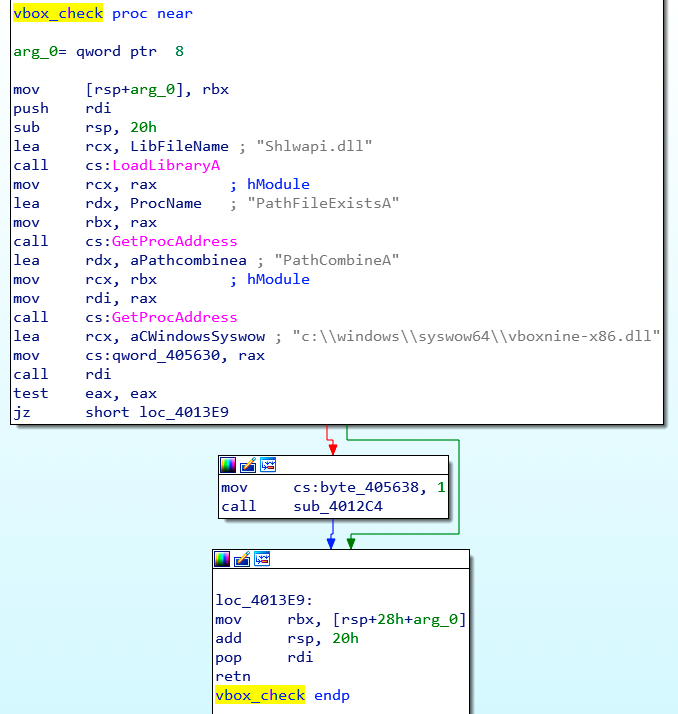
\includegraphics[width=\linewidth]{media/vbox_check.png}
\caption{the check that looks for the VBox DLL}\label{vbox_check}
\end{figure}
\begin{markdown}

\end{markdown}
\begin{figure}[!htbp]
\centering
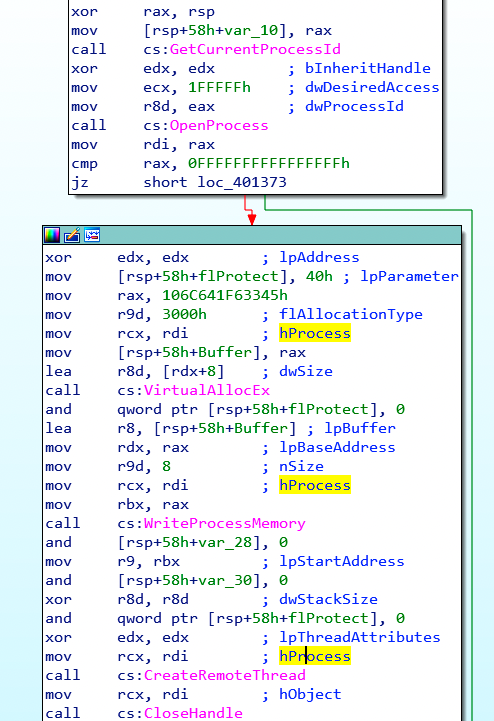
\includegraphics[width=\linewidth]{media/crash_code.png}
\caption{the code that ultimately throws an exception}\label{crash_code}
\end{figure}
\begin{markdown}

\clearpage
To bypass this (and other) checks we have a couple of options, among them:\s

* dirty hack: uninstall the Guest Additions or delete/rename the DLL 
* patch: change the string to a non-existing file
* patch: change the conditional jump for this check
* register manipulation: keep changing the zero flag to get past the crash code
* patch: **jump past the exception code in `sub_4012C4`** (the crash code)
    * this allows us to work around all checks with a single patch
    * the checks will still trigger but they won't throw an exception
    * I've chosen this option
    
---

\noindent I've patched the instruction at `0x4012FA` from `je 0x401373` to `jmp 0x401373`.
This effectively **always** jumps past the crash code allowing us to use the binary both inside and outside a VM and/or debugger.
\n
I think this is a rather clean solution but I've also mentioned possible other patches for all further checks.

---

\noindent Here is a binary diff via Radare2 that shows the entirety of the patch I've ended up with: Code \ref{radiff}.\n

\end{markdown}
\begin{lstlisting}[language=bash,name={binary diff},label={radiff}]
ben::cyric:shared:$ radiff2 -D Crypter_A.exe Crypter_A_betterpatch.exe
--- 0x000006fa  74
- je 0x79
- xor edx, edx
+++ 0x000006fa  eb
+ jmp 0x7b
+ xor edx, edx
\end{lstlisting}
\begin{markdown}

## Three More Protections Against Analysis

> \noindent Find three other ways that the executable tries to protect itself from manual analysis. Please explain them in detail and describe how you bypassed the protection measures.

* **delta time check** via `GetTickCount64()`s
    * this check actually starts before the check from the previous task
        * the current tick count is saved (`0x401409` and `0x40140`)
        * the first check is executed (`0x401412`)
        * the current tick count is saved again (`0x401417`)
        * the delta of the two counts is calculated and compared with 1000 ms (`0x40141D` to `0x401431`)
    * if it took longer (as when carefully stepping through the program) the check triggers
    * if you don't manually step through the program you don't have to patch this at all (it will only trigger if you take more than 1 second between the two calls to `GetTickCount64()`)
    * possible patch: increase the 1000 ms (`0x3E8`) to a higher value or patch the jump
* **`CheckRemoteDebuggerPresent()`**
    * called at `0x401455`
    * this checks if the process is attached to a debugger
    * the return value is tested for zero `0x40145B`
    * `0x40145D` jumps if it was non-zero (to the aforementioned crash code)
    * in conclusion: crash if the process is attached to a debugger
    * possible patch: nop out the call (`rax` is zero before it)
* I'm not sure what I would classify as the third additional countermeasure. Maybe the usage of the variable **`byte_405638`** to keep track of the outcome of the checks. All these checks are made inconsequential by my crash code patch.
Maybe stack cookies? But those are not really a hindrance since we're not writing a buffer overflow and have full control over them (and they are more of a compiler feature anyway). 
Or the `IsProcessorFeaturePresent` fastfail-check before the main (but that never gets executed and does not prevent analysis). Some dead code? I did not find a noticeable amount that would prevent analysis.
* Or maybe it's the fact that there is no Bitcoin address in sight, even though people are supposed to send some to get the key. That would certainly stump me as an analyst ;)
* I've spent so much time thinking about what the third protection mechanism might be; maybe it's the task itself. Very meta.

## Persistence

> \noindent Does the executable make itself persistent in the system? If so, please explain how.

\noindent There seems to be no persistence.

---

\noindent I could not find any persistence, neither by looking in the binary nor by fetching all processes with `tasklist` and diffing them with a known clean state.
I've also checked in the common places (registry, etc.) without avail.
\n
The binary does not seem to be set up for persistence either (e.g. by looking for new files and encrypting them as they are added).
Simply running the encryption on startup again would not make any sense either, since the encryption function is its own inverse function.

## Which Files Are Encrypted?

> Which files are encrypted? Please explain how you figured that out.

\noindent All the Python (`.py`) files in the `C:\Tools` folder. (Incidentally the file type I would least want to lose in a ransomware attack.)

---

\noindent I have figured this out early on since I usually take a look at all strings in a binary as one of the first steps. Here the globbing pattern and the path caught my eye. See Figure \ref{dstrings}.

\begin{figure}[!htbp]
\centering
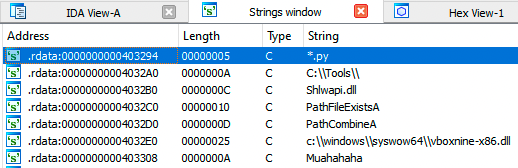
\includegraphics[width=\linewidth]{media/dstrings.png}
\caption{partial list of strings in malware}\label{dstrings}
\end{figure}

\noindent Looking for the occurrences of these two strings (via xrefs) quickly lead me to the piece of code that iterates over all files and directories in `C:\Tools` and the extension check (for Python files), which confirmed my suspicion. See Figure \ref{xrefs}.

\begin{figure}[!htbp]
\centering
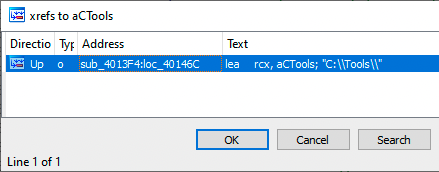
\includegraphics[width=\linewidth]{media/xrefs.png}
\caption{cross references for the `C:\Tools` variable}\label{xrefs}
\end{figure}

\noindent After patching the binary and running it I had further confirmations since all Python files in the Tools directory were indeed encrypted (and decrypted if run again).

## Parameters for `CreateFileA`

> \noindent There are two different calls to CreateFileA. Besides the filename parameter, please explain the parameters given to those two calls (value and meaning in your own words).

* the first call at `0x4010BB`
    * a pointer to the string of a python filename as `lpFileName`
    * `0x80000000` for `dwDesiredAccess`: **`GENERIC_READ`**
        * get read access to resource (Python file in our case)
        * to read the content (so it can xor/encrypt it)
    * `0x3` for `dwShareMode`: **`FILE_SHARE_READ`** plus **`FILE_SHARE_WRITE`**
        * to allow both read and write access rights to the file by other processes
    * `0x0` for `lpSecurityAttributes`, so **`NULL`**
        * the file handle can't be passed to a child processes
        * and the file gets a default security descriptor
    * `0x3` for `dwCreationDisposition` **`OPEN_EXISTING`**
        * this mode will throw an error if the file does not exist as opposed to silently creating it (**`ERROR_FILE_NOT_FOUND`**)
    * `0x8000000` for `dwFlagsAndAttributes`: **`FILE_FLAG_SEQUENTIAL_SCAN`**
        * used for sequential file access from beginning to end
        * this is used as a hint to Windows which helps it with optimizing caching behaviour
            * for example: no need to keep already read content in cache (because we're only moving forward)
    * for `hTemplateFile`
        * this is ignored because we're opening an existing file
    * if everything went allright we have a read handle now
* the second call at `0x4010F3`
    * this is executed if we got a valid (read) file handle from the previous call
    * same filename as the call preceding it
    * `0x40000000` for `dwDesiredAccess`: **`GENERIC_WRITE`**
        * now the malware actually wants to write the encrypted content
    * all the other parameters are the same as for the previous call
    * if everything worked we now have a valid write handle as well

## The Encryption Method

> \noindent Which encryption method is used? Please explain the piece of code responsible for it.

\noindent **The encryption method boils down to a bytewise XOR.**

---

\noindent The program iterates through all files and folders (skipping the current folder `.` and the parent folder `..`) looking for all python files along the way.  If one is found the absolute path to that file is concatenated and the address that points to that string is loaded into `rcx`. 
\n
Before the real encryption starts a bit of preparation happens, starting at `0x401000`:\s

* the encryption key is calculated and stored in `rsi` (see next section)
* a read and write handle is created (see previous section)

\noindent\s Now a single byte is read (at `0x40114B`).
\n 
\noindent **This single byte is `xor`ed with the calculated key at `0x40110E`:\s `xor     [rsp+160h+var_120], sil`**.
\n
This new encrypted byte is written back (in place) to the file at `0x40112C`:\s
`call    cs:WriteFile`.
\n
This repeats until the entire file is encrypted (and thus no more bytes can be read).
## The Encryption Key

> \noindent What's the encryption key being used for encryption? How is it calculated? 

The encryption key is 68, which is `0x44` or `0b1000100`.

---

\noindent The key is based on the username of the executing user which is fetched  via `call cs:GetUserNameA`.
\n
The following is an algorithm of how it is derived:\s

* get the username: `Analysis` (at `0x401040`)
* count chars in username string: `8` (1-indexed, `0x40104F` to `0x401055`)
    * by `inc`ing until we hit the string terminator
* add up all individual ASCII values (using our counter, `0x401064` to `0x401075`):
    * A: `0x41`
    * n: `0x6E`
    * a: `0x61`
    * l: `0x6C`
    * y: `0x79`
    * s: `0x73`
    * i: `0x69`
    * s: `0x73`
* which totals `0x344` in our case
* `AND` this value with `0x800000FF` (mask out, at `0x401077`)
    * keep only the leftmost (sign) and the 8 rightmost bits
* which gives us `0x44` our key!

---

The same in Python:

\end{markdown}
\begin{lstlisting}[language=python,name={key_calculator.py},label={keycalc}]
sum = 0
for c in 'Analysis': sum += ord(c)
hex(sum & 0x800000FF)  # '0x44'
\end{lstlisting}
\begin{markdown}

## Writing a Decryptor

> \noindent Share some piece of pseudo-code for a decryption tool that could be distributed to customers.

\noindent I've opted for Python instead of pseudo-code so I could test it and make sure not to forget any steps (plus it's fun to write). I've used Python 2 instead of 3 because that's the one that was available on the Windows box. See Code \ref{decryptor}. \n
This piece of code assumes that the customer has created a backup before running the decryptor in case anything goes wrong (and we want to build that habit for the future).

\end{markdown}
\begin{lstlisting}[language=python,name={decryptor.py},label={decryptor}]
#!/usr/bin/env python2
import os

path = 'C:\Tools'
filetype = '.py'
key = 0x44


def decrypt(filename):
    print 'decrypting ', filename
    decrypted = ''

    # read and decrypt content of file:
    with open(filename, 'rb') as file:
        for byte in file.read():
            decrypted += chr(ord(byte) ^ key)  # xor each byte with key.

    # write back decrypted content:
    with open(filename, 'wb') as file:
        file.writelines(decrypted)


# recursively iterate through path:
for subdir, dirs, files in os.walk(path):
    for filename in files:

        # decrypt affected files:
        if filename.endswith(filetype):
            decrypt(subdir + os.sep + filename)
\end{lstlisting}
